\chapter{Implicit-Transition Model for Three-dimensional Grain Growth}
\label{chap:implicit}

\lettrine{I}{n} a three-dimensional setting, grain boundaries are surfaces of polyhedra instead of curves delimiting a plain grain. 
Triple junctions are now triple lines where three grains meet. The single point where four grains meet are called quadruple junctions. 
Formally, consider a cube unit domain $[0,1]^3 \subset \mathbb{R}^3$ with periodic boundary conditions. 
Notation is similar to the two dimensional setting. Grains are still defined as a set $\grains $ of $N$ disjoint regions as \eqref{eq:grainsdef}, that is, a set of polyhedra. 
Let $\boundaries$ the set of grain boundaries delimiting the grains as in \eqref{eq:boundariesdef}, but now these are polygonal surfaces. 
Instead of triple junctions, we have the set $\vertices$ of $M$ quadruple junctions.

A classic approach for generating initial conditions for grain growth simulation consists in the Voronoi tessellation of a domain from a random set of initial points~\cite{Barmak2013,BarralesMora2008,Kinderlehrer2006,Lazar2011,Syha2010,torres2015}. 
The proposed model extends the idea of vertex-driven models to three dimensions by maintaining grain surfaces flat and triple lines straight during grain structure evolution. 
This implies that vertices can't be moved individually as vertex model works, otherwise grain surfaces will no longer remain flat. %would become curved. 
In order to impose these restrictions it is proposed to move the generator points used for the generation of the Voronoi tessellation instead. This implies that every time we move the generator points, we need to build a new tessellation. 
As the tessellation always gives flat surfaces, the imposed restriction of flat faces and straight triple lines are always accomplished~\cite{sazo2017implicit}.

The motivation for this model is that two dimensional topological transitions are already difficult to implement and check. Chapter~\ref{chap:parallelflip} shows how cumbersome can be this process even if we introduce sophisticated mechanisms. 
In a three dimensional setting the possibilities for topological transitions increases considerably since grain boundaries are now surfaces instead of curves~\cite{BarralesMora2008}. 
This model handles implicitly topological transitions, that is, to avoid modifications, consistency checking and repairs to underlying data structure, only relying in how the structure is generated via tessellations.

The tessellation is build using a certain group of points in the domain. Let $\mathcal{P}$ the set of generator points of a tessellation such that:
\begin{equation*}
    \mathcal{P} = \mathcal{P}(t) = \{ \mathbf{P}^{(1)}, \mathbf{P}^{(2)}, \dotsc, \mathbf{P}^{(N)} \}.
\end{equation*}
Grain structure evolves when generator points moves and each new tessellation after generator motion is considered a new state of the grain structure. 
This continuous motion and tessellations are stable in front of small changes of the generator points~\cite{reem2011geometric}. 
Grain removal is assumed to happen when a grain decreases its volume until a certain minimum value is reached. 
The grain is removed by simply removing the related generator point.

The total energy of the system is inspired in the total energy of a two dimensional grain structure from \eqref{eq:energy} where instead of integrating along curve grain boundaries, we integrate over grain surfaces.
\begin{equation}
    E(t) = \sum_{k=1}^{K} \int_{\Gamma^{(k)}} \sigma_k\,dA,
    \label{eq:energy3d}
\end{equation}
where $\sigma^{(k)}$ is the grain boundary energy per unit of area, analogously to $\gamma$ in the two dimensional setting. 
In order to simulate the grain structure evolution we must ensure that \eqref{eq:energy3d} decreases. The following velocity equation is proposed for the generator points:
\begin{equation}
    \dot{\mathbf{P}}^{(\grn)} = \sum_{m=1}^{M} \gamma^{(m,l)}\mathbf{T}^{(m,l)},
    \label{eq:voronoivel}
\end{equation}
where $m$ and $l$ indicates quadruple junctions sharing a triple line, $\gamma^{(m,l)}$ is an energy term related to the triple line and $\mathbf{T}^{(m,l)}$ is the unit tangent vector to the triple line. 
Consider $\vertices_\grn,\, \grn = 1,\dotsc,N$ the set of all the quadruple junctions that belongs to a grain $\grn$. 
Each quadruple junction in $\vertices_\grn$ has four triple lines and thus four neighbor junctions, but only three of them lies in $\grn$, the other triple junction belongs to an adjacent grain $\grn'$, this is the considered triple line in \eqref{eq:voronoivel} between $m$ and $l$ and generates an unit tension $\mathbf{T}^{(m,l)}$ that will affect the motion of the generator point $\mathcal{P}^{(\grn)}$. Algorithm~\ref{alg:implicit} summarizes the proposed method.

\begin{algorithm}[t]
\caption{Implicit-transition Model for Grain Growth}
\label{alg:implicit}
\begin{algorithmic}[1]
\Procedure{Implicit\_Grain\_Growth}{$N_0, \Delta t$}
\State $t \gets$ $0$
\State $N(0) \gets$ $N_0$
\State $\mathcal{P}(t) \gets$ $N_0$ random points in unitary first octant.
%\While{stopping criteria not met}
\While{$80\%$ of the grains has not been removed}
\State $\grains(t) \gets$ Voronoi($\mathcal{P}(t)$).
\Comment{Grain structure}
\State $\grains(t) \gets \grains(t) \setminus \{\grn \in \grains(t) \mid \mbox{Volume}(\grn) < V_{\text{ext}}\}$
% remove grains uch that their volume is below $V_{\text{ext}}$
\State $\mathbf{F}(t) \gets$  Velocity for each generator point.
\State $\mathcal{P}(t+\Delta t) = \mathcal{P}(t) + \dot{\mathcal{P}}(t) \cdot \Delta t$
\State $t=t+\Delta t$
\EndWhile
\State \Return $\grains(t)$
\EndProcedure
\end{algorithmic}
\end{algorithm}

\section{Numerical Experiments}

In order to test the proposed model, two numerical experiments were performed. 
The first is related to how the evolution equation does indeed minimize the total energy of the grain structure. 
The second experiment shows that grains obtained in tessellations over time evolve and gain or lose faces through topological transitions that are not explicitly handled. 
Isotropic setting was chosen thus $\gamma^{(m,l)} = 1$ for all triple lines.

\subsection{Energy Minimization}

Recall that the proposed energy equation in \eqref{eq:voronoivel} is not derived from the total energy in \eqref{eq:energy3d}.
Total energy over time is shown in Figure~\ref{fig:3D_energy}. 
This model still achieves a decreasing energy behavior. 
Although the outcome is not monotonically decreasing, it is asymptotically decreasing.

We found out that if we move the generator points using a linear combination of the the unit outer normal vectors of the faces $\N$, that is
%
\begin{equation}
    \dot{\mathbf{P}}^{(\grn)} = \sum_{\bnd^{(k)} \in \grn} \sigma_k \mathbf{N}_k,
    \label{eq:voronoivel2}
 \end{equation}
%
we can effectively decrease the total energy of the system monotonically during some range of time in simulation. Figure~\ref{fig:3D_energy_improved} shows the total energy over time for this evolution equation with $\sigma_k = 1$. This is a new proposal that needs to be studied further.

\begin{figure}
    \centering
    \subfloat[Total energy of a three-dimensional simulation with the Implicit-transition model.]{
        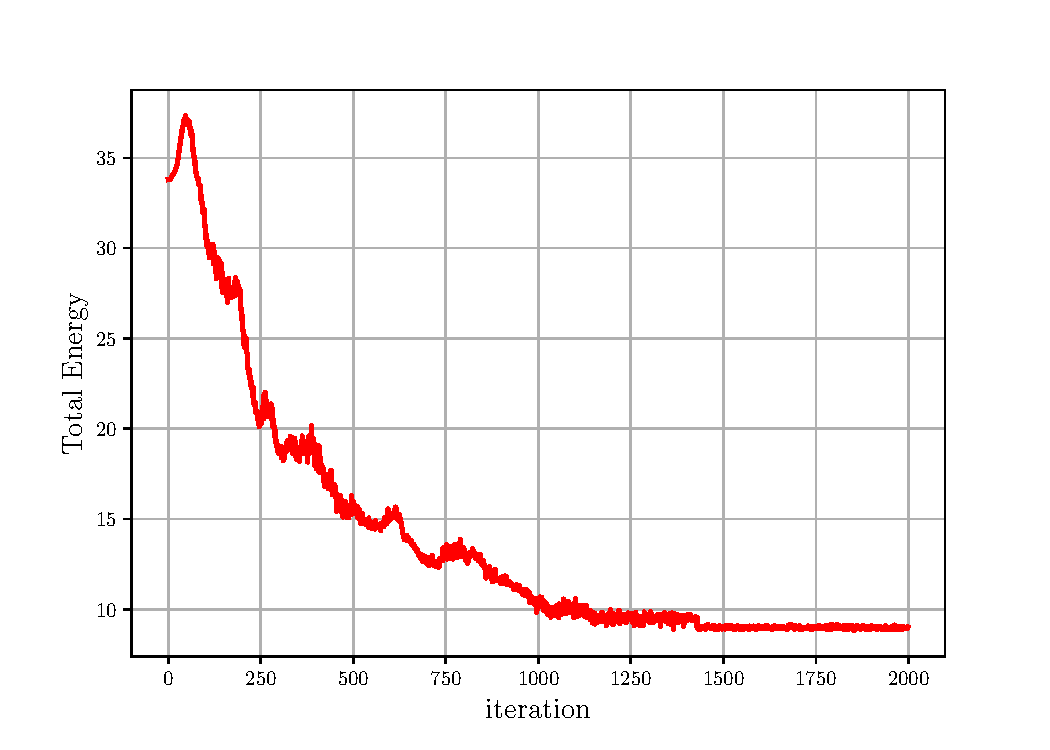
\includegraphics[scale=0.6]{figures/3d_voronoi/3D_energy.pdf}
        \label{fig:3D_energy}
    }\\
    \subfloat[Total energy of a three-dimensional simulation with the Implicit-transition model with the normal vectors evolution equation.]{
        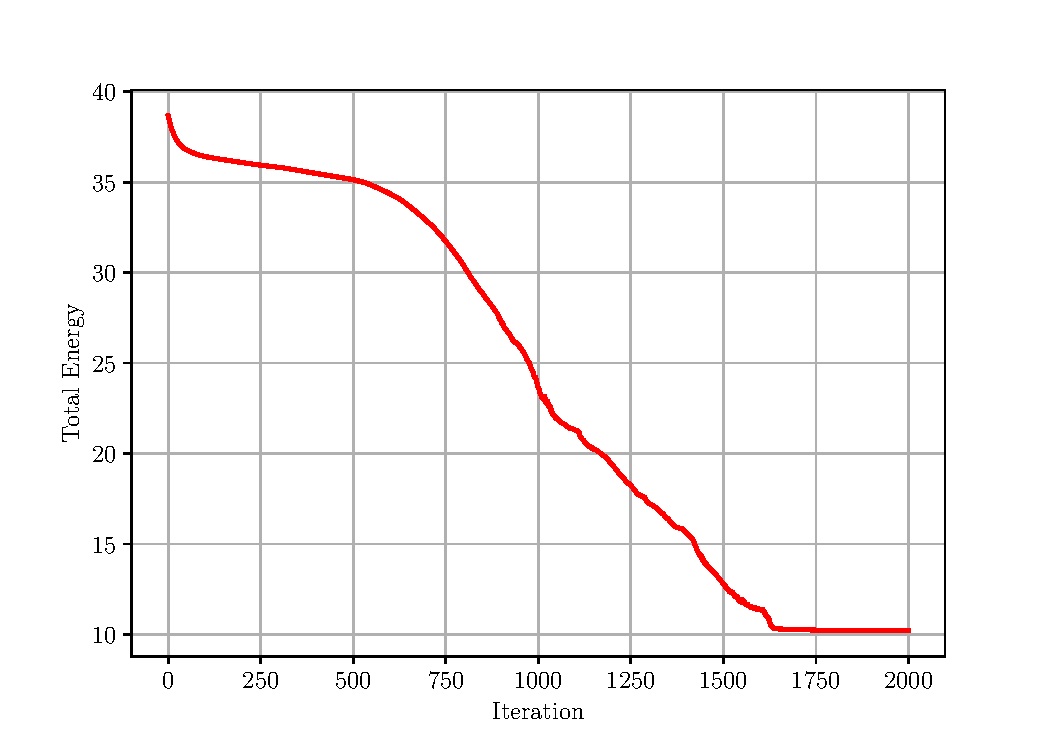
\includegraphics[scale=0.6]{figures/3d_voronoi/3D_energy2.pdf}
        \label{fig:3D_energy_improved}
    }
    \caption{Total energy of three-dimensional Models: Implicit-transition Model and evolution with normal vectors.}
\end{figure}

\subsection{Topological Transitions}
The algorithm successfully handles triple lines flippings, surface transitions, and grain removals.
Notice that the topology of the grain structure could be complex but the algorithm is still able to manage the  topological changes since this is done by Voronoi tessellation itself.
A grain boundary flipping is shown in \figurename~\ref{fig:3Dflipping}.
A triple line begins to shrink
(\figurename~\ref{flip1}), 
then it collapses into a single point 
(\figurename~\ref{flip2}), 
and finally this unstable configuration evolves generating a new triple line (\figurename~\ref{flip3}).

\begin{figure*}[!t]
    \centering
    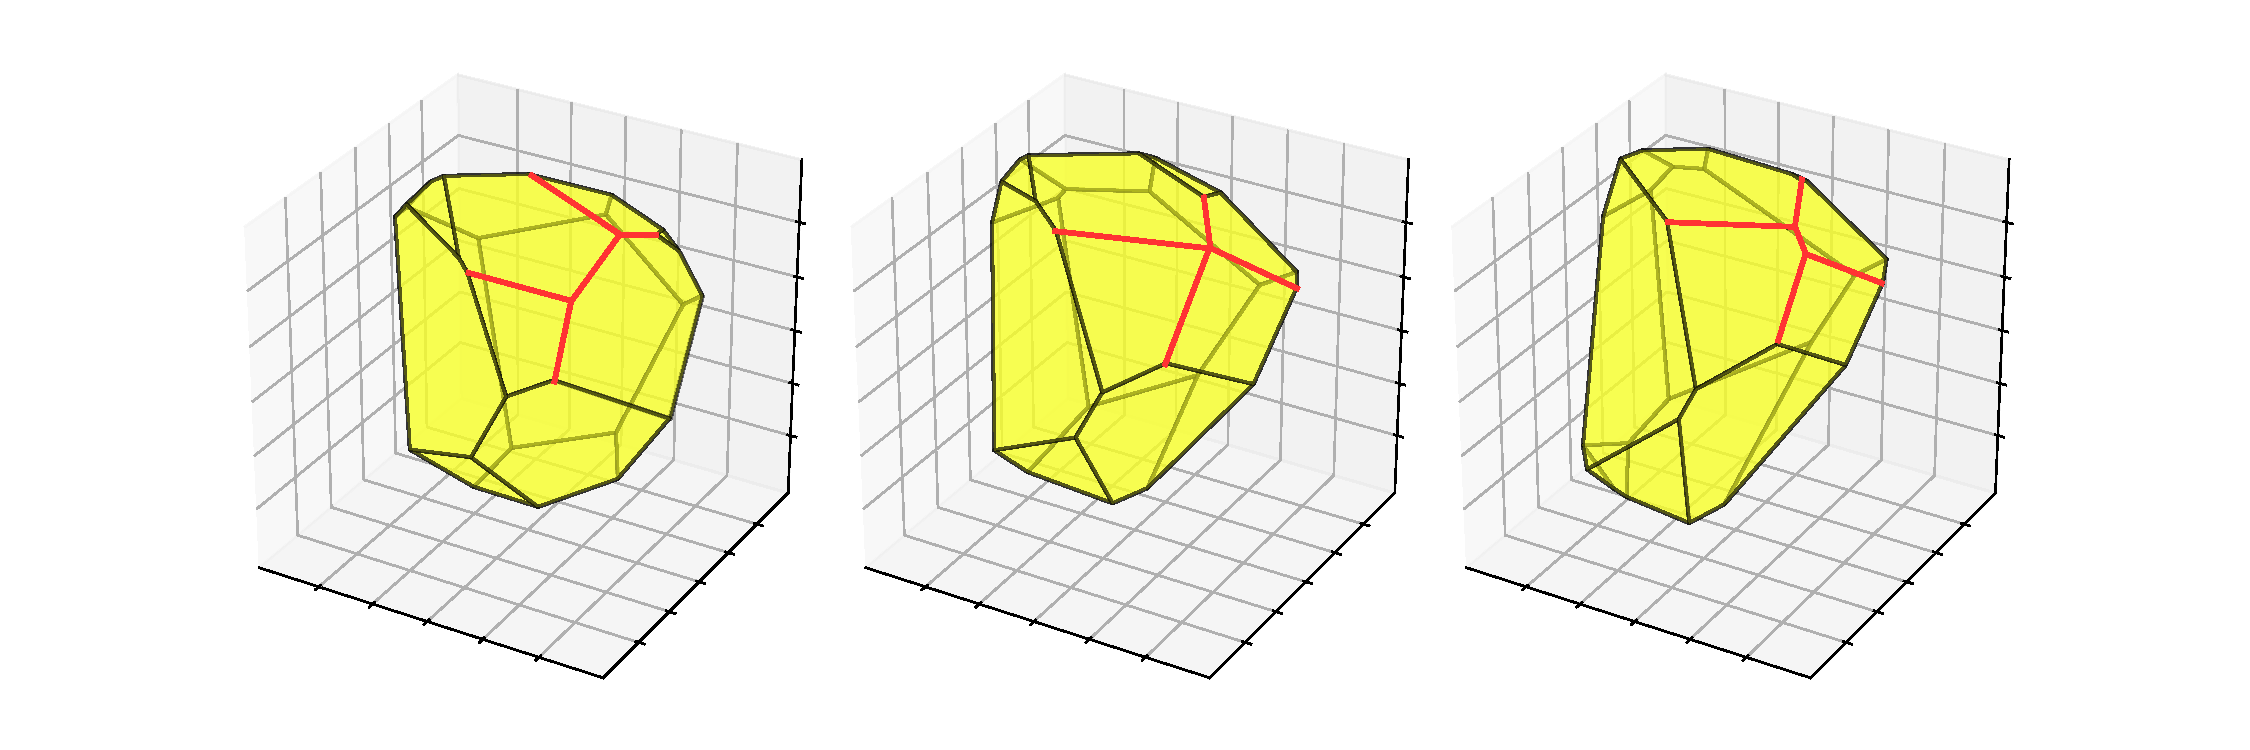
\includegraphics[trim={0 2em 0 2em},scale=0.37]{figures/3d_voronoi/3D_flipping.pdf}
    \subfloat[\label{flip1}]{\hspace{.2\linewidth}}
    \subfloat[\label{flip2}]{\hspace{.2\linewidth}}
    \subfloat[\label{flip3}]{\hspace{.2\linewidth}}
    \caption[Flipping scheme on a single three-dimensional grain.]{Flipping scheme on a single three-dimensional grain. 
    Some triple lines and neighbor grains are omitted.}
    \label{fig:3Dflipping}
\end{figure*}


\figurename~\ref{fig:3Dfaceremoval} shows a surface
transition. A surface begins to reduce its area (\figurename~\ref{rem1}, \ref{rem2}) until it becomes a vertex (\figurename~\ref{rem3}).

\begin{figure*}[!t]
    \centering
    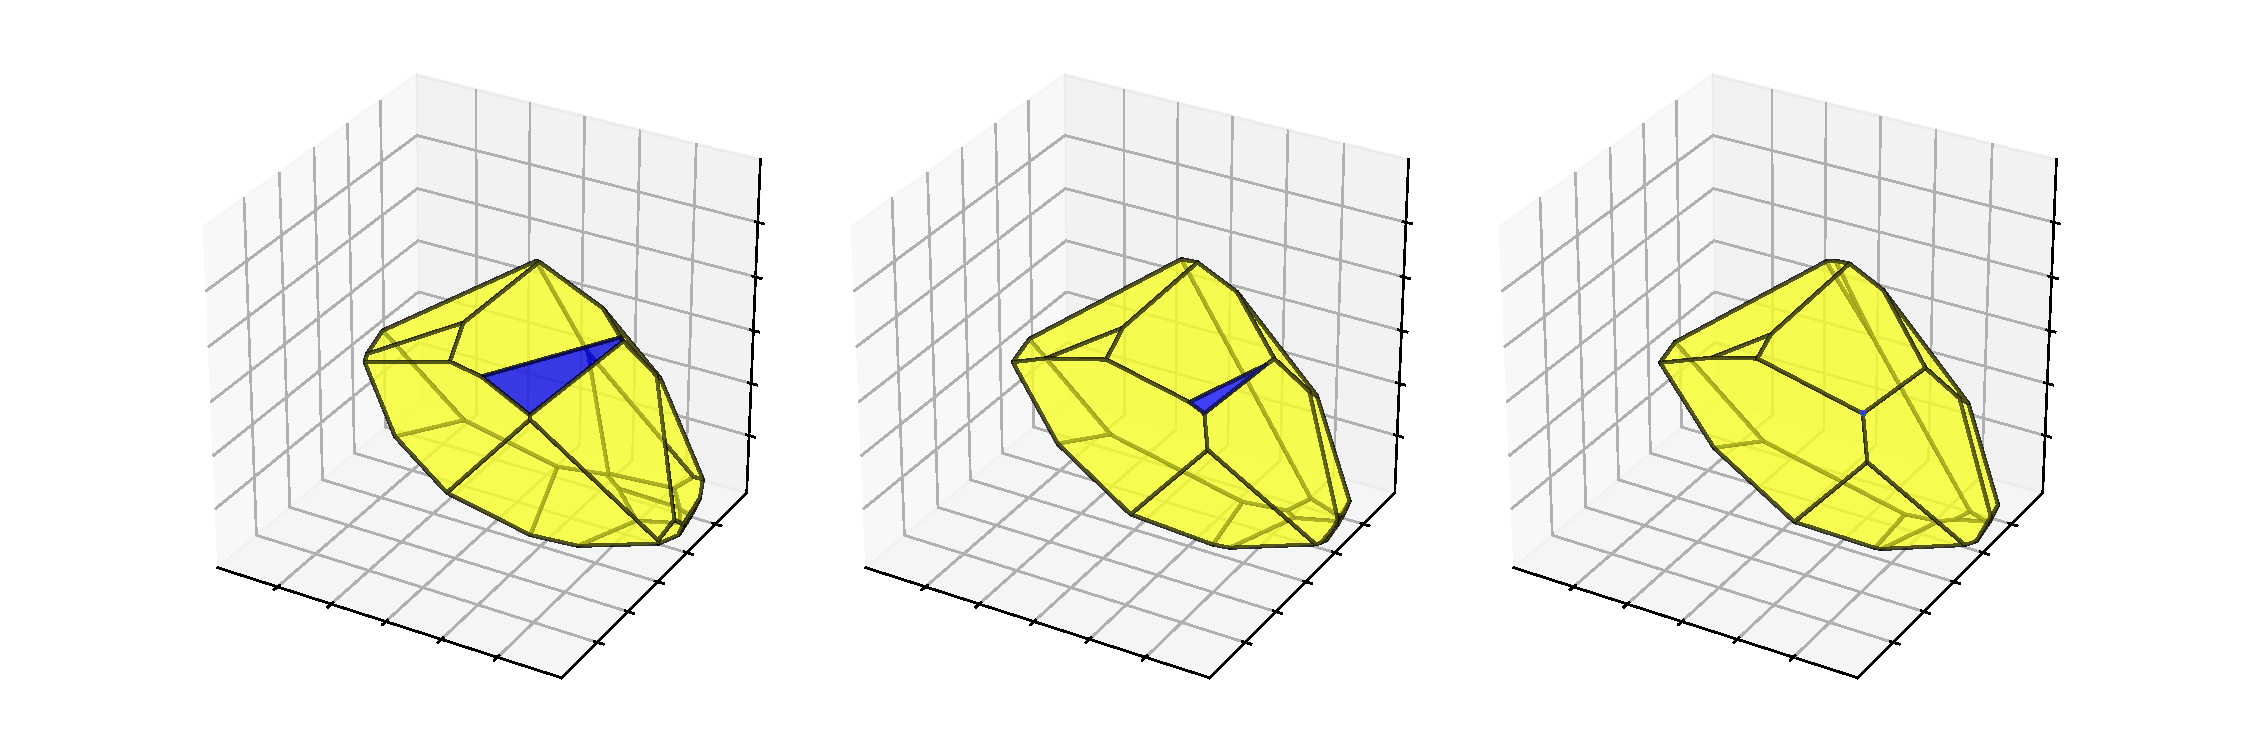
\includegraphics[trim={0 2em 0 2em},scale=0.37]{figures/3d_voronoi/3D_surface_removal.pdf}
    \subfloat[\label{rem1}]{\hspace{.2\linewidth}}
    \subfloat[\label{rem2}]{\hspace{.2\linewidth}}
    \subfloat[\label{rem3}]{\hspace{.2\linewidth}}
    \caption[Surface transition in a three-dimensional grain]{Surface transition in a three-dimensional grain. Triple lines of other related grains are omitted.}
    \label{fig:3Dfaceremoval}
\end{figure*}

Finally grains removal are also observed, 
see \figurename~\ref{fig:3Dremoval}. 
The grain reduces its volume from 
$V\approx 5\cdot10^{-4}$ to $V \approx 1.2\cdot10^{-4}$ until the threshold $V_{\text{ext}}$ is reached with $V \approx 9.6\cdot10^{-5}$. 
In experiments $V_{\text{ext}}$ is set between $10^{-4}$ and $10^{-5}$.

\begin{figure*}[!t]
    \centering
    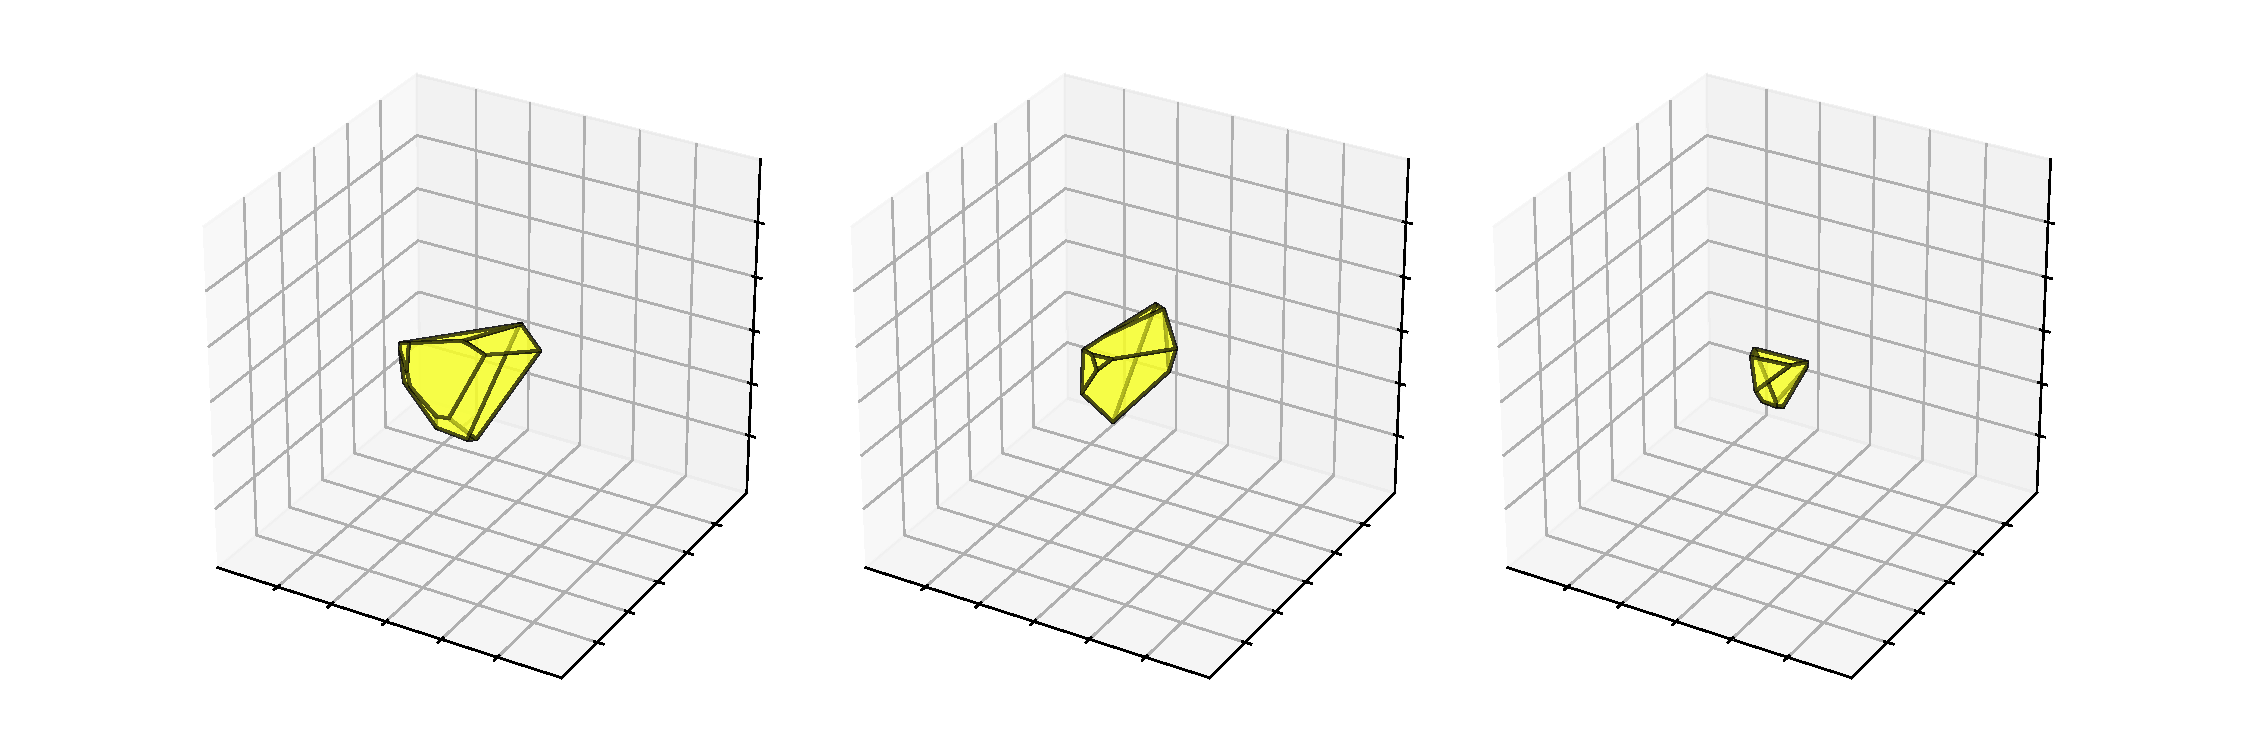
\includegraphics[trim={0 2em 0
    2em},scale=0.37]{figures/3d_voronoi/3D_grain_removal.pdf}
    \subfloat[\label{grem1}]{\hspace{.2\linewidth}}
    \subfloat[\label{grem2}]{\hspace{.2\linewidth}}
    \subfloat[\label{grem3}]{\hspace{.2\linewidth}}
    \caption[Three-dimensional grain removal]{Grain removal stages. 
    The grain loses boundaries (surfaces) until its
    volume is less than $V_{\text{ext}}$.
    Then the grain is removed by means of 
    removing its generator point.}
    \label{fig:3Dremoval}
\end{figure*}
